% -*- coding: utf-8 -*-
% !TEX-encoding = UTF-8


\documentclass[a4paper]{article}
\usepackage[utf8]{inputenc}
\usepackage[english,italian]{babel}
\usepackage[colorlinks]{hyperref}
\usepackage{graphicx}
\usepackage[output-decimal-marker={,}]{siunitx}
\usepackage{booktabs}

\begin{document}
\title{Elaborato di Interazione Uomo Macchina}
\author{Michele Scala \\ Giacomo Annaloro}
\date{20 gennaio 2015}
\maketitle


\section{Introduzione}
Questo progetto per il corso di Interazione Uomo Macchina costituisce un esperimento per valutare la leggibilità del testo nelle interfacce utente, al variare dei colori usati. Il programma è costituito da due test distinti ognuno a sua volta formato da due pannelli strutturati in modo analogo e differenziati solo per i colori.
I task corrispondenti ai due test sono rispettivamente:
\begin{enumerate}
\item individuare una data parola tra un insieme disordinato;
\item contare le occorrenze di un certo termine in un dato testo.
\end{enumerate}
Per ogni run l'ordine di presentazione dei test è casuale, in modo da non essere influenzata dalla preparazione dell'utente. 
Il parametro valutato per entrambi i task è il tempo impiegato per portarli a termine.

\section{Realizzazione}
Il programma è realizzato sulla piattaforma Qt. 
La gestione dell'esecuzione è affidata alla classe \verb:MainWindow:, che implementa una finestra che può contenere un oggetto \verb:QWidget: e un pulsante per passare alla schermata successiva. In base ai segnali che essa riceve, detemina quale test (e in particolare quale pannello appartenente a quel test) mostrare fino all'ultimo di riepilogo, che per elencare i dati raccolti si serve della classe \verb:Result:.
\verb:MainWindow: si occupa anche del calcolo del tempo trascorso da quando un pannello di un test è mostrato a quando il timer viene resettato per il passaggio alla finestra successiva.

\section{Test 1}
Il test 1 verifica la percezione del colore e il pre-attentive processing mostrando un insieme disordinato di parole di due colori diversi e chiedendo l'individuazione di una di queste.
Le parole sono implementate da \verb:QPushButton: senza bordi, disposti disordinatamente all'interno del \verb:QWidget: principale. Il testo dei vari pulsanti è generato leggendo il file \verb:wordslist.txt: e la parola da selezionare è scelta casualmente all'interno della lista.
La classe grafica che realizza il pannello è \verb:Panel1Test1: e viene istanziata con due diverse combinazioni di colori.
La figura ~\ref{figura:dialogo1} ne illustra un esempio.

\begin{figure}[http]
\centering
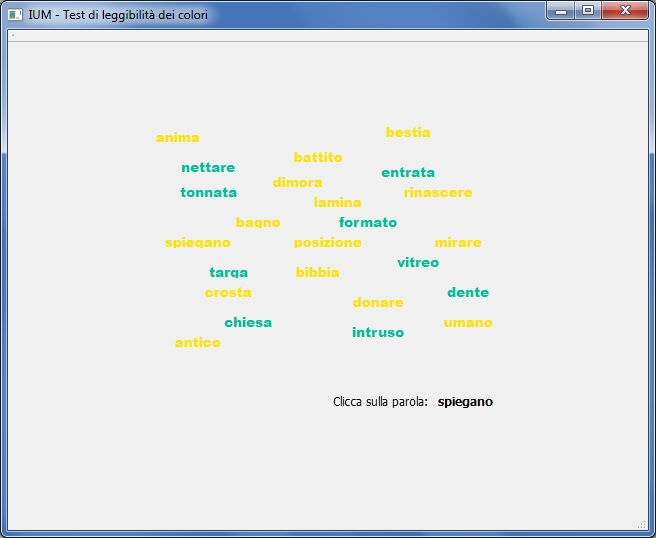
\includegraphics[width=0.65\textwidth]{dialogo2}
\caption{Un pannello del Test 1}
\label{figura:dialogo2}
\end{figure}

I colori usati nel test con relativi parametri sono riportati in tabella ~\ref{tabella:colori}.

\begin{table}
\centering
\begin{tabular}{lrrr}
\toprule
Colore & {Hue} & {Sat} & {Val} \\
\midrule
Giallo 		& 53	& 255 & 255	\\
Azzurro	& 168	& 255	& 190	\\
\midrule
Blu 		& 224	& 255 & 255 \\
Rosso 	& 0	& 202	& 190	\\
\bottomrule

\end{tabular}
\caption{Specifica dei colori usati nel Test 1}
\label{tabella:colori}
\end{table}

Come si può vedere per entrambi i pannelli sono stati scelti colori con valori molto elevati sia per saturazione che per luminosità. Inoltre per ciascuna delle due combinazioni è stata mantenuta costante la differenza tra tali valori e quelli dello sfondo.
A variare notevolmente è invece la tonalità:
\begin{itemize}
\item nel primo caso sono usati \emph{giallo} e \emph{azzurro}: due colori sottrattivi chiari caratterizzati da uno scarso contrasto con lo sfondo, che quindi rendono le parole confondibili con esso;
\item nel secondo caso sono usati \emph{blu} e \emph{rosso}: due colori additivi e primari, ben distinguibili dallo sfondo, ma che rendono più difficoltosa la lettura dei caratteri. Proprio il blu e il rosso infatti, sono considerati accostati insieme i meno indicati per la leggibilità del testo. Oltre al fatto che sono entrambi saturi, il blu è da preferire per gli sfondi.
\end{itemize}

\section{Test 2}


\begin{figure}[http]
\centering
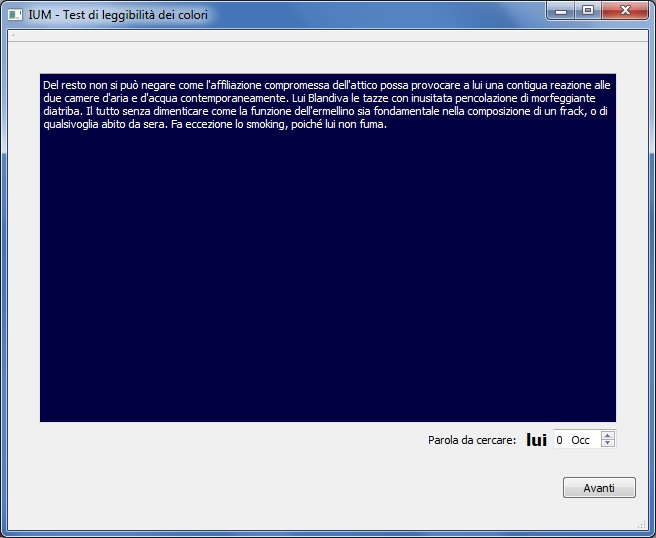
\includegraphics[width=0.65\textwidth]{dialogo1}
\caption{Un pannello del Test 2}
\label{figura:dialogo1}
\end{figure}


\section{Risultati}

\begin{table}
\centering
\begin{tabular}{lSS}
\toprule
Run & {Test 1} & {Test 2} \\
\midrule
1971 & 203.2	& 0	\\
1976 & 289.6	& 0	\\
1986 & 812		& 0	\\
2001 & 1754.34	& 0	\\
2005 & 1824.51	& 454.62 \\
2008 & 1527.16	& 804.05 \\
2012 & 1024.94 	& 1014.61 \\
\midrule
Media & 4 & 5 \\
\bottomrule

\end{tabular}
\caption{Riepilogo dei risultati (tempi in millisecondi)}
\label{tabella:risultati}
\end{table}


\end{document}